  \subsection{Medición de la tensión eficaz de una onda proveniente de un circuito de control de ángulo de conducción}
Para la siguiente parte del experimento, se utiliza un control de medición 
de ángulo de disparo, circuito que se enseña en la Figura \ref{fig:CircuitoTriacDiac}.

% \ref{fig:CircuitoTriac}.

% \begin{figure}[H]
%   \centering
%   \frame{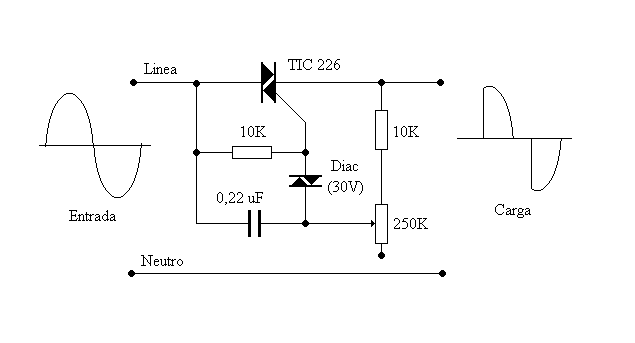
\includegraphics[width=0.6\textwidth]{Imagenes/ActividadPractica/MedicionDeTensionEficazConCircuitoTriac/Esquema_Circuito_Angulo_Disparo.png}}
%   \caption{Esquema del circuito de control de ángulo de disparo.}
%   \label{fig:CircuitoTriac}
% \end{figure}

El procedimiento consiste en medir la tensión de entrada al circuito, 
y medir la de salida sobre la carga, tomando lecturas
al variar el ángulo de conducción con un multímetro que mide True RMS y otro de valor medio. 
Luego, se debe confeccionar un gráfico normalizado de tensión de salida 
respecto de la entrada, con las curvas obtenidas con cada instrumento.

El esquema de conexión se presenta a continuación en la Figura \ref{fig:EsquemaConexionTriac}.

\begin{figure}[H]
  \centering
  \frame{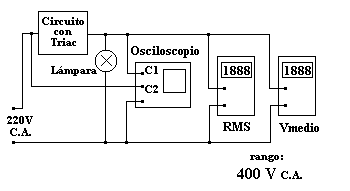
\includegraphics[width=0.4\textwidth]{Imagenes/ActividadPractica/MedicionDeTensionEficazConCircuitoTriac/Esquema_Conexion_Circuito_Angulo_Disparo_2.png}}
  \caption{Esquema de conexión para el relevamiento de curva.}
  \label{fig:EsquemaConexionTriac}
\end{figure}

Se presentan a continuación en la Tabla~\ref{tab:TablaExp2} los valores tabulados. Se debe tener en cuenta que, debido al circuito de disparo, nunca se logra obtener el ángulo de disparo 0º.

\begin{table}[H]
\centering
  \begin{tabular}{|c|c|c|c|c|}
    \hline
      \textbf{Fase} & $\mathbf{Vo_1~[V]}$ & $\mathbf{Vo_2~[V]}$ & $\mathbf{(\frac{Vo_1}{V_{in}})}$ & $\mathbf{(\frac{Vo_2}{V_{in}})}$ \\
    \hline
      0°    & -       & -       & -       & -           \\
      36°   & 222,8   & 211,6   & 1,013   & 0,962\\
      72°   & 194,5   & 158,6   & 0,884   & 0,721\\
      108°  & 135,8   & 189,6   & 0,617   & 0,407\\
      144°  & 58,77   & 30,0    & 0,267   & 0,136\\
      180°  & 0       & 0       & 0       & 0\\
    \hline
  \end{tabular}
\caption{Tabla de valores obtenidos.}
\label{tab:TablaExp2}
\end{table}

      \begin{figure}[H]
        \centering
        \begin{subfigure}[ht]{0.48\textwidth}
          \frame{\includegraphics[width=\textwidth]{Imagenes/ActividadPractica/MedicionDeTensionEficazConCircuitoTriac/Exp2_AnguloDisparo36º.png}}
          \caption{Ángulo de 36°.}
        \end{subfigure}
        \hfill 
        \begin{subfigure}[ht]{0.48\textwidth}
          \frame{\includegraphics[width=\textwidth]{Imagenes/ActividadPractica/MedicionDeTensionEficazConCircuitoTriac/Exp2_AnguloDisparo72º.png}}
          \caption{Ángulo de 72°.}
        \end{subfigure}
        \begin{subfigure}[ht]{0.48\textwidth}
          \frame{\includegraphics[width=\textwidth]{Imagenes/ActividadPractica/MedicionDeTensionEficazConCircuitoTriac/Exp2_AnguloDisparo108º.png}}
          \caption{Ángulo de 108°.}
        \end{subfigure}
        \hfill 
        \begin{subfigure}[ht]{0.48\textwidth}
          \frame{\includegraphics[width=\textwidth]{Imagenes/ActividadPractica/MedicionDeTensionEficazConCircuitoTriac/Exp2_AnguloDisparo144º.png}}
          \caption{Ángulo de 144°.}
        \end{subfigure}
        \begin{subfigure}[ht]{0.48\textwidth}
          \frame{\includegraphics[width=\textwidth]{Imagenes/ActividadPractica/MedicionDeTensionEficazConCircuitoTriac/Exp2_AnguloDisparo180º.png}}
          \caption{Ángulo de 180°.}
        \end{subfigure}

        \caption{Medición de tensión eficaz para distintos ángulos de conducción.}
         \label{fig:MedicionAnguloConduccion}
      \end{figure}

Finalmente, se confecciona un gráfico con los valores obtenidos, 
donde se visualizan las curvas de los instrumentos, cuyos valores 
son relativos al valor medido de la red, que en éste caso corresponde 
con 234~V eficaces.

\begin{figure}[H]
  \centering
  \frame{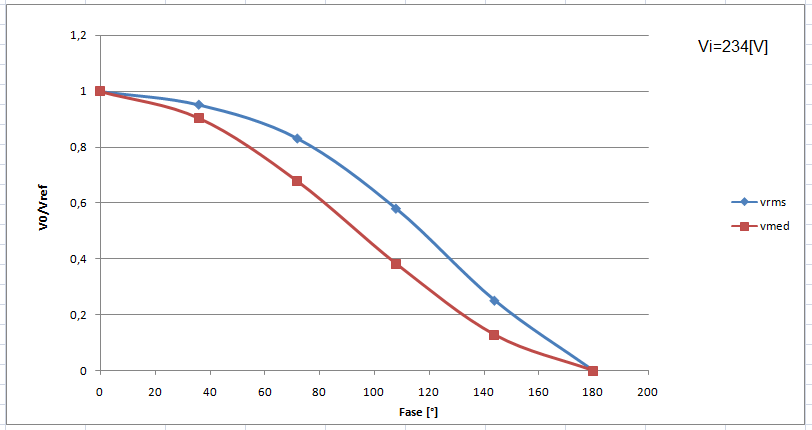
\includegraphics[width=0.8\textwidth]{Imagenes/ActividadPractica/MedicionDeTensionEficazConCircuitoTriac/Grafico_Contrastacion_2.png}}
  \caption{Gráfico obtenido.}
  \label{fig:CurvaTrueMedio}
\end{figure}
